\subsection{Summary of the chapter}

In this chapter, the characteristic structure of the solution of hyperbolic problems in elastic-plastic solids in two space dimensions has been highlighted.
It is known since the 50s that plastic flow in two-dimensional solids yields two families of waves whose speeds depend on the stress state, the slow and fast waves.
In addition, these plastic waves may have an impact on all stress components in contrast to elastic discontinuities, hence the name of combined-stress waves.
During the 60s, attention has been paid to simple waves in particular two-dimensional problems thus providing, among others, solutions of Picard problems in an elastic-plastic medium undergoing step loadings \cite{Clifton,Ting68,Ting73}.
% Idem pour ting ? c'est dit dans l'intro ? voir ce qui est fait dans le 73
The singular nature of such problems lies in the fact that the characteristic structure of the solution depends on the external loading undergone.
Indeed, it has been shown \cite{Clifton} that boundary conditions can lead to plastic flow involving one fast, one slow, or both simple waves.
Therefore, it is crucial to be able to identify typical stress paths followed in each simple wave in order to link the initial data to a given stress state, and subsequently to determine the occurring wave pattern.

%Besides these works, investigations on plastic shocks have been carried out.
%The existence of such solutions is due to the state law for the hydrostatic pressure which dominates deviatoric effects.


$\newline$
%% Lin et Ballman
Based on these works, an iterative Riemann solver \cite{Lin_et_Ballman}, whose procedure has been recalled in section \ref{sec:stress_paths_num}, has been developed for the numerical solution of the thin-walled tube problem. 
This solver relies on the ability to connect a stationary state to initial data by a characteristic wave pattern.
% L'idée ici c'est de généraliser cette approche pour tous les problèmes 2D
Following this approach, identifying characteristic wave patterns for general elastoplastic problems in two space dimensions should allow to enrich the numerical solution with the knowledge of physics.
For that purpose, the characteristic analysis of two-dimensional problems in elastic-plastic materials with linear isotropic hardening under plane strain and plane stress, in projection in an arbitrary direction of space, has been carried out in section \ref{sec:charac_plast}.
Fast and slow waves are also involved in the solution so that applying the method of characteristic through the simple waves provides a system of ODEs.
Integration of this system leads to integral curves in terms of velocity and stress components that are followed inside the combined-stress waves.
%Integration of this system leads to combined stress paths that are followed between initial and final stress states on the one hand, and to the integral curves in terms of velocity components involving integral along those loading paths on the other hand.
Specializing the ODEs to one direction of a Cartesian grid, it has been shown in section \ref{sec:stress_paths} that the loading paths satisfied through slow and fast waves are perpendicular in the stress space for both plane strain and plane stress.
Moreover, it has been established that the stress paths exhibit particular behavior in the space $(\sigma_{11},\sigma_{22},\sigma_{12})$, that is $d\sigma_{11}=0$, $d\sigma_{12}=0$ or $d\sigma_{22}=0$, for special values of the components of the acoustic tensor.
These situations are achieved for different stress states depending on whether the problem involves plane stresses of plane strains as shown in section \ref{sec:stress_paths}.

$\newline$
The complexity of the ODEs derived in section \ref{sec:charac_plast} prevents identifying all the singularities which may occur along the loading paths.
Hence, the mathematical analysis has been supplemented with numerical results consisting of the integration of stress paths from arbitrary initial stress values lying on the initial yield surface, for the particular direction $\vect{e}_1$.

%% Thin-walled tube
First, in section \ref{sec:num_thin-walled} the loading paths resulting from the integration of the ODEs derived in section \ref{sec:charac_plast} have been compared to those of Clifton \cite{Clifton}.
The two different formulations, respectively based on elastoplastic stiffnesses and softnesses, show  good agreement.

%% Cont. planes
Second, the evolution of stress components across fast and slow waves under plane stress has been looked at in section \ref{sec:num_plane_stress}.
It appears that though the loading paths are rather complex in stress space through a fast wave, the stress evolution in the deviatoric plane is restricted to the initial yield surface until one direction of pure shear is reached.
A singularity then occurs so that the numerical integration cannot be pursued.
On the other hand, the loading paths resulting from the integration of ODEs satisfied inside a slow wave exhibit complex shapes along which $\sigma_{11}$ varies much less than the other stress components.

%% Def. planes
Third, the plane strain case has been considered in section \ref{sec:num_plane_strain}.
Once again, the integral curves inside a fast wave show complex shapes in stress space, and an evolution restricted to the initial yield surface in the deviatoric plane.
In that case, however, the paths may follow a direction of pure tension/compression in the latter plane so that the plastic flow is radial for high values of the hardening modulus. 
In contrast, the paths inside slow waves first rotate on the yield surface and then lead to a stress state of pure shear in the deviatoric plane.

\subsection{Towards a two-dimensional elastoplastic Riemann solver}
The physical structures emphasized in this chapter enable a better understanding of the propagation of waves in two-dimensional elastoplastic media, although further investigations are required.
On the other hand, the loading paths followed in fast and slow simple waves can be used in order to improve the numerical simulation of these problems.

%% Lin et Ballman
One possibility is to generalize the approach proposed by Lin and Ballman \cite{Lin_et_Ballman} based on the clues provided above.
The idea would be to successively assume stationary states of the Riemann problem in terms of stress $\sigma_{11}$, $\sigma_{12}$ and $\sigma_{22}$ in order to build stress paths starting from the initial data.
Namely, considering the direction $\vect{e}_1$, the loading paths followed through a slow wave can be integrated backward starting from the guessed state.
Then, different situations may occur:
\begin{itemize}
\item[(1-a)] the curve thus obtained crosses the initial yield surface at a point where $\sigma_{22}$ satisfies the initial data.
  In that case, the elastic discontinuities led to that stress state so that the characteristic structure corresponds to that depicted in figure \ref{fig:charac}\subref{subfig:charac1}.
\item[(1-b)] if on the other hand the point reached on the initial yield does not satisfy the initial stress $\sigma_{22}$, a fast wave is added in order to browse the initial yield surface until the initial data is recovered.
  This situation is depicted in figure \ref{fig:charac}\subref{subfig:charac2}.
\item[(2-a)] the curve resulting from the reverse integration across a slow wave intersects the plane $\sigma_{12}=0$.
  Then, assuming that the paths of slow waves are symmetric with respect to that plane, a fast wave is added in order to reach the initial yield surface at the initial value of $\sigma_{22}$.
  Indeed, the fast waves have been shown to yield horizontal paths in the ($\sigma_{11},\sigma_{12}$) plane, in such a way that only that type of wave enables the achievement of the initial elastic domain.
  This also corresponds to figure \ref{fig:charac}\subref{subfig:charac2}.
\item[(2-b)] if at last, the guessed state is such that $\sigma_{12}=0$, a fast wave allows reaching the initial yield surface as depicted in figure \ref{fig:charac}\subref{subfig:charac3}.
\end{itemize}

\begin{figure}[h!]
  \centering
  \subcaptionbox{One slow wave \label{subfig:charac1}}{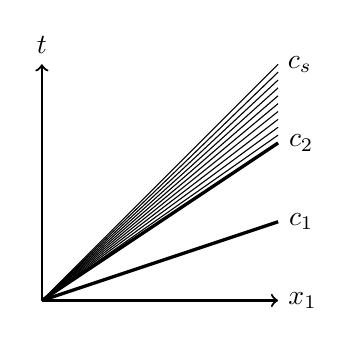
\begin{tikzpicture}
    \draw[thick, ->] (0,0) -- (3.,0) node [right] {$x_1$};
    \draw[thick, ->] (0,0) -- (0,3) node [above] {$t$};
    \draw[very thick] (0,0) -- (3,1) node [right] {$c_1$};
    \draw[very thick] (0,0) -- (3,2) node [right] {$c_2$};
    \foreach \x in {0.1,0.2,...,0.9}
    \draw (0,0) -- (3,2+\x);
    \draw (0,0) -- (3,3) node [right] {$c_s$};
\end{tikzpicture}} \qquad 
  \subcaptionbox{Both simple waves \label{subfig:charac2}}{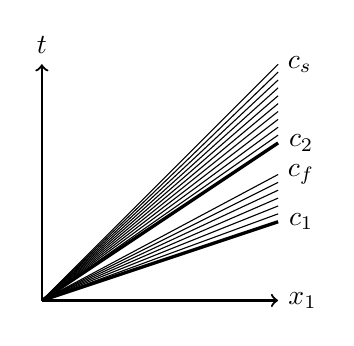
\begin{tikzpicture}
    \draw[thick, ->] (0,0) -- (3.,0) node [right] {$x_1$};
    \draw[thick, ->] (0,0) -- (0,3) node [above] {$t$};
    \draw[very thick] (0,0) -- (3,1) node [right] {$c_1$};
    \foreach \x in {0.1,0.2,...,0.5}
    \draw (0,0) -- (3,1+\x);
    \draw (0,0) -- (3,1.6) node [right] {$c_f$};
    \draw[very thick] (0,0) -- (3,2) node [right] {$c_2$};
    \foreach \x in {0.1,0.2,...,0.9}
    \draw (0,0) -- (3,2+\x);
    \draw (0,0) -- (3,3) node [right] {$c_s$};
\end{tikzpicture}} \qquad 
  \subcaptionbox{One fast wave \label{subfig:charac3}}{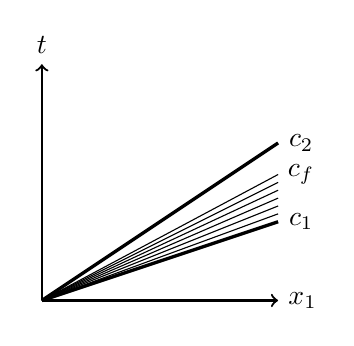
\begin{tikzpicture}
    \draw[thick, ->] (0,0) -- (3.,0) node [right] {$x_1$};
    \draw[thick, ->] (0,0) -- (0,3) node [above] {$t$};
    \draw[very thick] (0,0) -- (3,1) node [right] {$c_1$};
    \foreach \x in {0.1,0.2,...,0.5}
    \draw (0,0) -- (3,1+\x);
    \draw (0,0) -- (3,1.6) node [right] {$c_f$};
    \draw[very thick]  (0,0) -- (3,2) node [right] {$c_2$};
    
\end{tikzpicture}}
  \caption{Characteristic structures possibly occurring in two-dimensional elastic-plastic solids.}
  \label{fig:charac}
\end{figure}
Notice however that the above elementary loading paths are based on strong assumptions about the symmetry of the loading paths that have not been shown so far.
As a result, additional work must be performed in order to develop this approach and to introduce it in numerical methods.
Moreover, the hardening of the material may modify the behavior of the loading paths and have not been considered yet.
At last, the generalization of the approach followed in this chapter to more complex hardening models (kinematic, nonlinear etc.) and other yield surfaces would be very interesting for the understanding of the physics. 

%%% Local Variables:
%%% mode: latex
%%% TeX-master: "manuscript"
%%% End:
